\documentclass[tikz]{standalone}
\usetikzlibrary{shapes}
\begin{document}
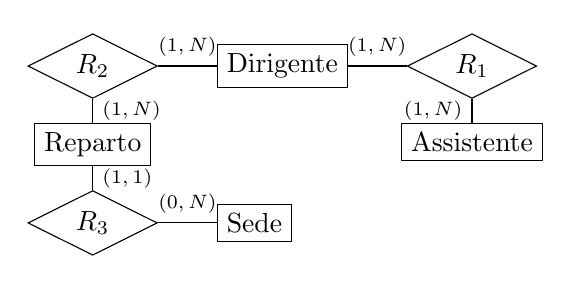
\begin{tikzpicture}
    \draw

    %%* Attributi:
    %%  node[draw, circle, inner sep=1pt, fill=black]{}node[right]{\footnotesize A}
    %%? Distanza orizzontale: E -(0.25,0.x)- A
    %%? Distanza verticale: E -(0,x * 0.22)- A

    %%* Cardinalità:
    %%  node[below right]{\scriptsize $(0,N)$}
    %%  node[above right]{\scriptsize $(0,N)$}
    %%  node[midway, above]{\scriptsize $(0,N)$}

    %%* Relazione:
    %%  node[draw, diamond, shape aspect=2, inner sep=3pt, anchor=90](r1){}
    %%  node[draw, diamond, shape aspect=2, inner sep=0.2pt, anchor=180](r2){R2}

    %%* Entità:
    %%  node[draw, rectangle, anchor=90](e1){}
    %%? Distanza verticale: E -(0.3)- R -(0.3) E
    %%? Distanza orizzontale: E -(0.75)- R -(0.75)- E

    (0,0)node[draw, rectangle, anchor=90](e1){Assistente}
    (e1.90)--++(0,0.3)node[draw, diamond, shape aspect=2, inner sep=3pt, anchor=270](r1){$R_1$}node[midway, left]{\scriptsize $(1,N)$}
    (r1.180)--++(-0.75,0)node[draw, rectangle, anchor=0](e1){Dirigente}node[midway, above]{\scriptsize $(1,N)$}
    (e1.180)--++(-0.75,0)node[draw, diamond, shape aspect=2, inner sep=3pt, anchor=0](r1){$R_2$}node[midway, above]{\scriptsize $(1,N)$}
    (r1.270)--++(0,-0.3)node[draw, rectangle, anchor=90](e1){Reparto}node[midway, right]{\scriptsize $(1,N)$}
    (e1.270)--++(0,-0.3)node[draw, diamond, shape aspect=2, inner sep=3pt, anchor=90](r1){$R_3$}node[midway, right]{\scriptsize $(1,1)$}
    (r1.0)--++(0.75,0)node[draw, rectangle, anchor=180](e1){Sede}node[midway, above]{\scriptsize $(0,N)$}
    ;
\end{tikzpicture}
\end{document}